%----------------------------------------------------------------
%
%  File    :  survey-taxonomy.tex
%
%  Author  :   Lukas Auer, David Heidinger, Nina Tschikof and Christina Vogel, TU Graz, Austria
% 
%  Created :  06 May 2026
% 
%  Changed :  08 May 2026
% 
%----------------------------------------------------------------

\chapter{Taxonomy of Dishonest Chart Techniques}
\label{chap:Taxonomy}

This chapter presents a taxonomy of dishonest chart techniques. The 9 identified techniques can be broadly grouped based on the type of manipulation they apply, including data selection, data aggregation, visual encoding, and the representation of uncertainty.

While each technique operates differently, they all share the common goal of influencing how viewers perceive and interpret data. The following sections describe each technique in more detail.

\newpage
\section{Cherry Picking}
Cherry picking is a form of selection bias where only a subset of available data is presented, while other relevant portions are deliberately or unintentionally left out. This practice is particularly problematic in time-series data, where the choice of start and end points can significantly influence the perceived direction and magnitude of a trend. By selecting intervals that support a specific narrative, the visualisation may suggest patterns that are not really representative of the full dataset \cite{cairo2019}.

From a cognitive perspective, viewers tend to interpret the presented data as complete and representative, especially when no indication of omitted information is provided. This can lead to too much trust in the observed chart and reduces the likelihood that viewers will question the underlying data selection process. As a result, cherry picking can effectively distort the interpretation without altering the actual data values, which makes this technique subtle but powerful.

\begin{figure}[htbp]
    \centering
    \includesvg[width=0.8\textwidth]{images/cherry_picking}
    \caption[Climate Reconstruction Chart]{Chart recreated from original in Python by the authors. \\
    Judd, E. J., Tierney, J. E., Lunt, D. J., Montañez, I. P., Huber, B. T., Wing, S. L., \& Valdes, P. J. (2024). A 485-million-year history of Earth’s surface temperature. Science, 385(6715). https://doi.org/10.1126/science.adk3705}
    \label{fig:cherry_picking}
\end{figure}

\newpage
\section{Underbinning}
Underbinning occurs when a chart, such as a histogram or a heatmap, uses too few bins to group the data. By dividing the dataset into overly broad intervals, the true shape of the distribution is hidden from the viewer. This reduction in detail obscures important features of the data, such as local clusters, gaps, and outliers. For example, if a dataset contains significant variations but is grouped into only a few coarse categories, the viewer will only see a very simplified picture.

When viewing an underbinned chart, people often assume that the displayed blocks accurately reflect how the data is actually spread out. Because the visual representation looks complete and valid, viewers might not realize that crucial details have been smoothed over. This can lead to a misunderstanding of the actual situation, as the chart might suggest a uniform trend where there is actually a lot of variation. Ultimately, while the raw data itself remains correct, the way it is grouped misleads the viewer by taking away the necessary context to understand the full dataset.

\begin{figure}[htbp]
    \centering
    \begin{minipage}{0.48\textwidth}
        \centering
        \includesvg[width=\linewidth]{images/proper_binning}
    \end{minipage}\hfill
    \begin{minipage}{0.48\textwidth}
        \centering
        \includesvg[width=\linewidth]{images/underbinning}
    \end{minipage}
    \caption[Comparison showing proper binning (left) versus underbinning (right).]{Chart recreated from original in Python by the authors. \\ FlowingData. Dishonest Charts, from https://flowingdata.com/projects/dishonest-charts/}
    \label{fig:binning_comparison}
\end{figure}

\newpage
\section{Axis Truncation}
Axis truncation is a technique where the baseline of a chart, most commonly the y-axis, does not start at zero. Instead, the axis is cut off to begin at a value much closer to the actual data points. Because the bottom portion of the chart is removed, the remaining visual space is stretched out to fill the area. 

The primary effect of this manipulation is that it makes small differences between values appear much larger than they really are. When people look at visualisations like bar charts, they naturally compare the physical heights of the bars to understand the data. If the baseline is missing, a minor increase might make one bar look twice as tall as another, even if the actual difference is very small. While the numbers written on the axis are still technically correct, the visual representation greatly exaggerates the situation and easily misleads the audience.

\begin{figure}[htbp]
    \centering
    \includesvg[width=0.7\textwidth]{images/axis_truncation}
    \caption[Fox News Tax Cuts Broadcast (2012).]{Chart recreated from original in Python by the authors. \\ Fox News Network. (2012, August 1). If Bush tax cuts expire [Television broadcast]. Media Matters for America. https://peoplesgdarchive.org/item/10481/if-bush-tax-cuts-expire-fox-news-infographic}
    \label{fig:axis_truncation}
\end{figure}

\newpage
\section{Artificial Flattening or Steepening}
Artificial flattening or steepening happens when the visual dimensions of a chart are stretched or compressed to change how the data looks. This is often done by using extreme aspect ratios or by setting an overly broad y-axis. For example, if the y-axis covers a much larger range of numbers than the actual data points need, a moving trend line will look completely flat. On the other hand, stretching the chart vertically can make small, slow changes look like very steep and sudden spikes or drops.

When people look at line charts, they naturally judge the importance of a trend by the steepness of the line. If a chart is artificially flattened, viewers might think a significant trend is just a minor detail and nothing to worry about. If the chart is steepened, a normal change can quickly look like a dramatic event. The actual data points remain exactly the same in both cases, but manipulating the visual boundaries of the chart completely alters the message the audience takes away from it.

\begin{figure}[htbp]
    \centering
    \begin{minipage}{0.48\textwidth}
        \centering
        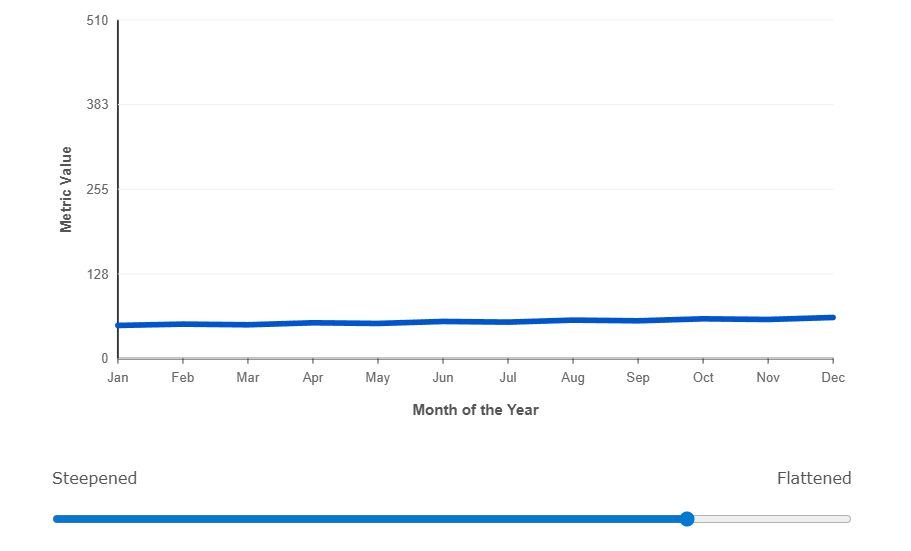
\includegraphics[width=\linewidth]{images/Artifical_Flattening_demo_example.png}
    \end{minipage}\hfill
    \begin{minipage}{0.48\textwidth}
        \centering
        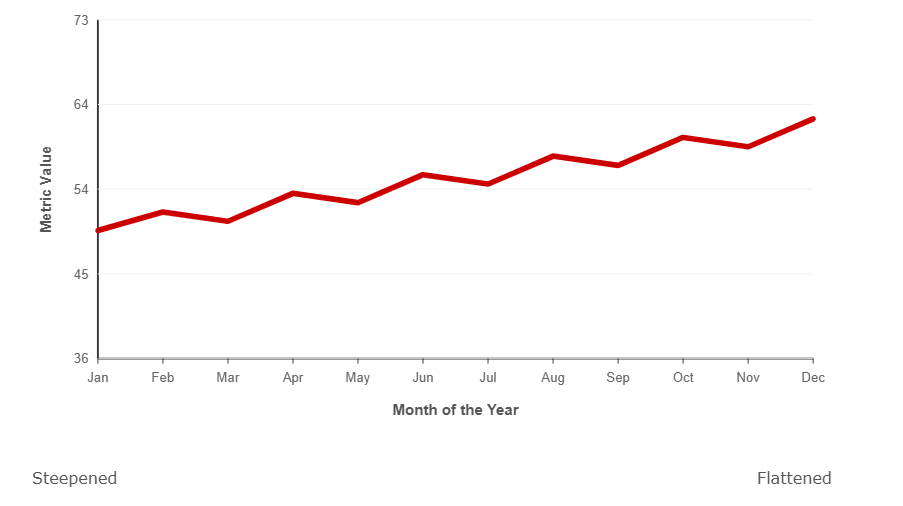
\includegraphics[width=\linewidth]{images/Artifical_Steepening_demo_example.png}
    \end{minipage}
    \caption[Comparison showing artificial flattening (left) versus steepening (right).]{Comparison showing artificial flattening (left) versus steepening (right). \\ Screenshot created by authors from the interactive demo.}
    \label{fig:flattening_steepening}
\end{figure}

\newpage
\section{Time Gap}
The time gap technique occurs when irregular or uneven time intervals are placed on a chart but are spaced out as if they were completely even. For example, a chart might show data points for the years 2020, 2021, and 2025 right next to each other, with the exact same amount of physical space between them. 

This manipulation effectively hides specific periods of time from the viewer. Usually, the years that are deleted are times when the data was stagnant or moving in an unwanted direction. When people look at a timeline or a trend chart, they naturally assume that time moves forward at a constant rate. Because the remaining data points are spaced evenly, the trend looks very smooth and continuous. The viewer is misled into seeing a steady development that did not actually happen in reality, simply because the missing time gaps are not visually shown.

\begin{figure}[htbp]
    \centering
    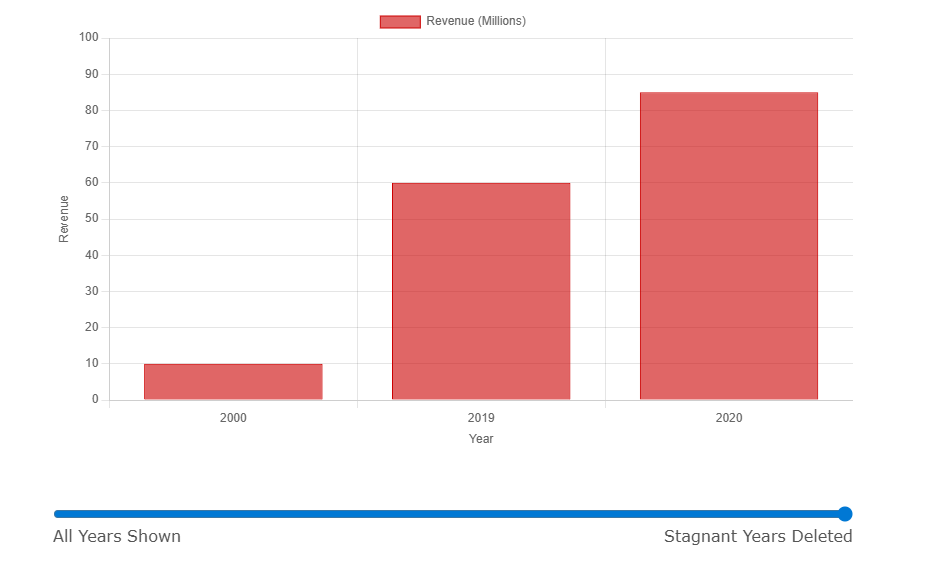
\includegraphics[width=0.8\textwidth]{images/Time_Gap_demo_example.png}
    \caption[Time Gap example.]{Screenshot created by authors from the interactive demo.}
    \label{fig:time_gap}
\end{figure}

\newpage
\section{Oversmoothing}
Oversmoothing happens when aggressive smoothing algorithms or over-fitted curves are applied to a set of raw data points. Instead of showing the actual data with all its natural ups and downs, the chart draws a very smooth and simple line. This technique hides critical short-term fluctuations, volatility, and local extremes that are actually present in the dataset.

When people look at an oversmoothed chart, they see a very clear and stable trend. Because the sudden spikes and sharp drops almost completely disappear, the viewer might think the situation is much more stable than it really is. While some smoothing can be a helpful tool to understand long-term developments, using it too heavily takes away important local patterns. This easily misleads the audience by making a highly variable and unpredictable dataset look perfectly calm and steady.

\begin{figure}[htbp]
    \centering
    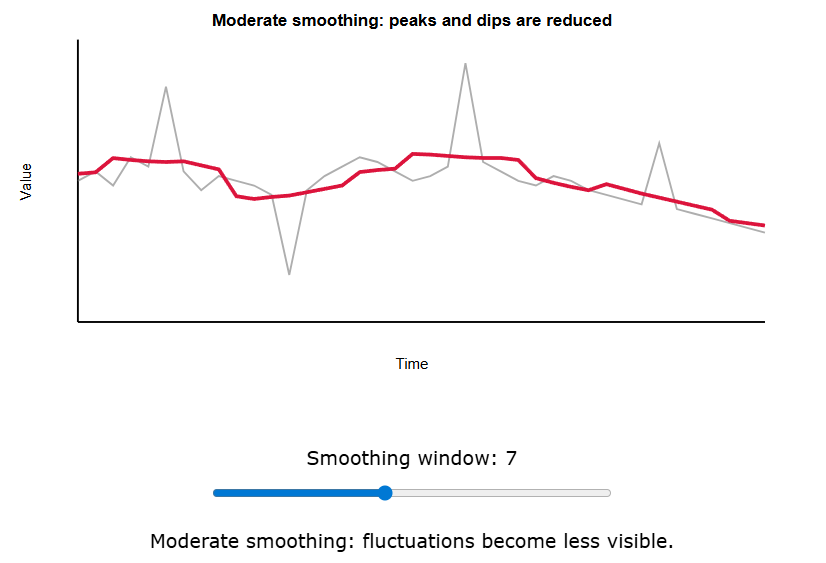
\includegraphics[width=0.8\textwidth]{images/Oversmoothing_demo_example.png}
    \caption[Comparison Original Data versus Oversmoothed.]{Screenshot created by authors from the interactive demo.}
    \label{fig:oversmoothing}
\end{figure}

\newpage
\section{Manipulating the Visual Encoding}
Manipulating the visual encoding happens when the choice of how to show data, such as using size, shape, or colour, is used to mislead the viewer. Instead of presenting the numbers clearly, the design uses confusing or exaggerated visual cues. For example, a chart might use a confusing colour scale or map a simple one-dimensional number to the two-dimensional area of an icon. 

When people look at these visualisations, their eyes naturally react to things like the overall size of a shape or bright, changing colours. If a number drops by half, but the overall area of the drawing is reduced to a quarter of its original size, the viewer will think the drop is much more dramatic than it actually is. 

\begin{figure}[htbp]
    \centering
    \includesvg[width=0.46\textwidth]{images/manipulating_the_visual_encoding_1}
    \caption[Shrinking Family Doctor]{Chart recreated from original in Python by the authors. \\ Time Magazine. (1990). The Shrinking Family Doctor [Data visualization]. InfoVis Wiki: The Lie Factor. Retrieved from https://infovis-wiki.net/wiki/Lie\_Factor}
    \label{fig:visual_encoding_1}
\end{figure}

\noindent Similarly, using a rainbow colour palette for simple continuous data can create false boundaries and patterns that do not exist in reality. This easily changes how the audience understands the data without altering the actual values.

\begin{figure}[htbp]
    \centering
    \begin{minipage}{0.48\textwidth}
        \centering
        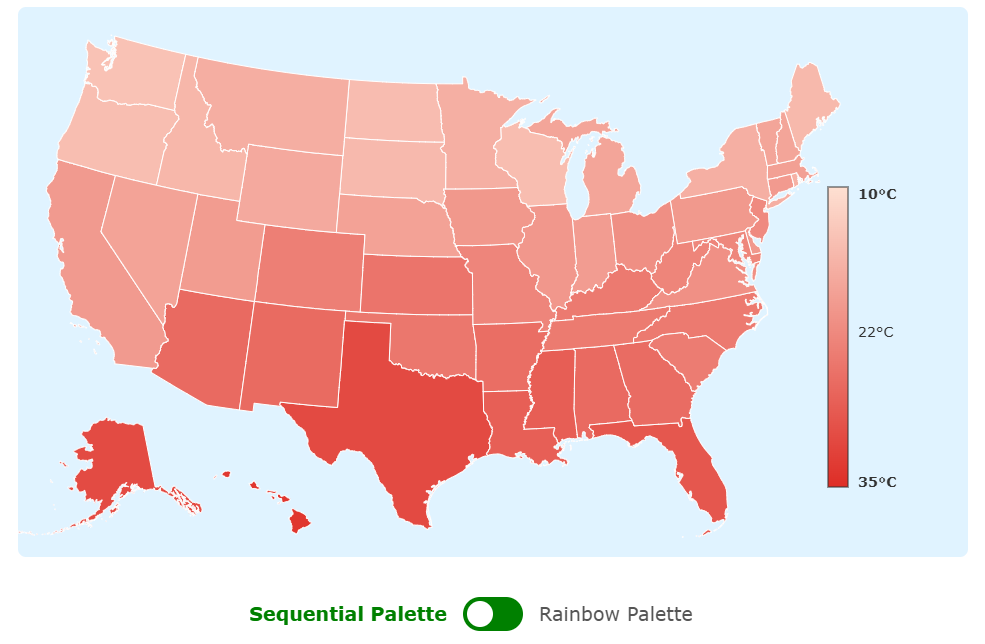
\includegraphics[width=\linewidth]{images/Visual_Encoding_2_sequential_demo_example.png}
    \end{minipage}\hfill
    \begin{minipage}{0.48\textwidth}
        \centering
        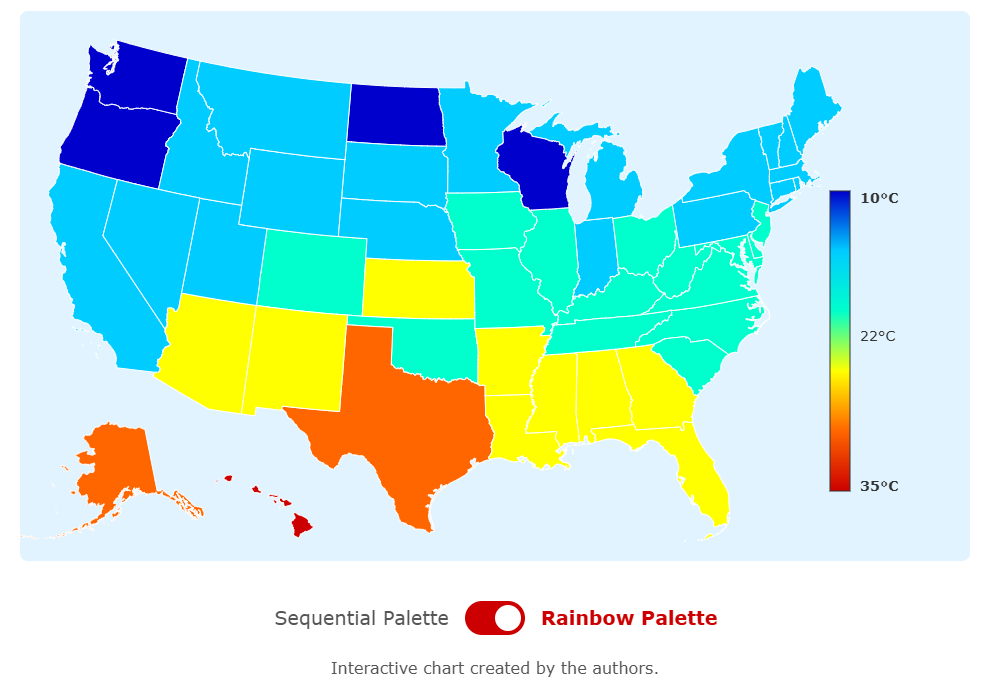
\includegraphics[width=\linewidth]{images/Visual_Encoding_2_rainbow_demo_example.png}
    \end{minipage}
    \caption[Comparison showing a sequential colour palette (left) versus a misleading rainbow palette (right).]{Screenshot created by authors from the interactive demo.}
    \label{fig:visual_encoding_2}
\end{figure}

\newpage
\section{Perspective Distortion}
Perspective distortion occurs when three-dimensional effects are improperly used in a two-dimensional visualisation, such as a pie chart. By tilting the chart backwards, the parts of the chart that are located in the front appear much closer to the viewer, while the parts in the back seem further away. 

This tilt creates a false sense of size and importance. Because of how 3D perspective works, a slice in the foreground will look physically larger than a slice in the background, even if its actual data value is smaller. For example, a 19.5\% share placed at the front of a tilted pie chart can easily look bigger than a 21.2\% share placed at the back simply because of the angle. When people look at a 3D chart, it becomes very difficult for them to compare the true angles and areas accurately. Ultimately, adding an unnecessary third dimension does not provide any new information, but it heavily distorts the true proportions and misleads the audience.

\begin{figure}[htbp]
    \centering
    \includesvg[width=0.6\textwidth]{images/perspective_distortion}
    \caption[Apple Macworld Keynote (2008).]{Chart recreated from original in Python by the authors. \\ Apple (2008, January 15). Macworld San Francisco 2008 Keynote Address [Presentation slide]. Macworld Conference \& Expo. Retrieved from https://paragraft.wordpress.com/tag/infovis/}
    \label{fig:perspective_distortion}
\end{figure}

\newpage
\section{Concealing Uncertainty}
Concealing uncertainty happens when a chart does not include important visual indicators of variance, such as error bars or confidence intervals. Instead of showing the possible range of a value, the visualisation only displays a single, exact line or data point. 

This technique suggests absolute precision in data that is actually just an estimate or a forecast. When people look at a projected trend without any signs of uncertainty, they naturally assume the future outcome is completely guaranteed. Because the potential error or variance is hidden from the screen, the viewer is misled into trusting the exact numbers too much. In reality, no forecast is perfect, but removing the visual boundaries of doubt creates a false sense of security and accuracy in the data.

\begin{figure}[htbp]
    \centering
    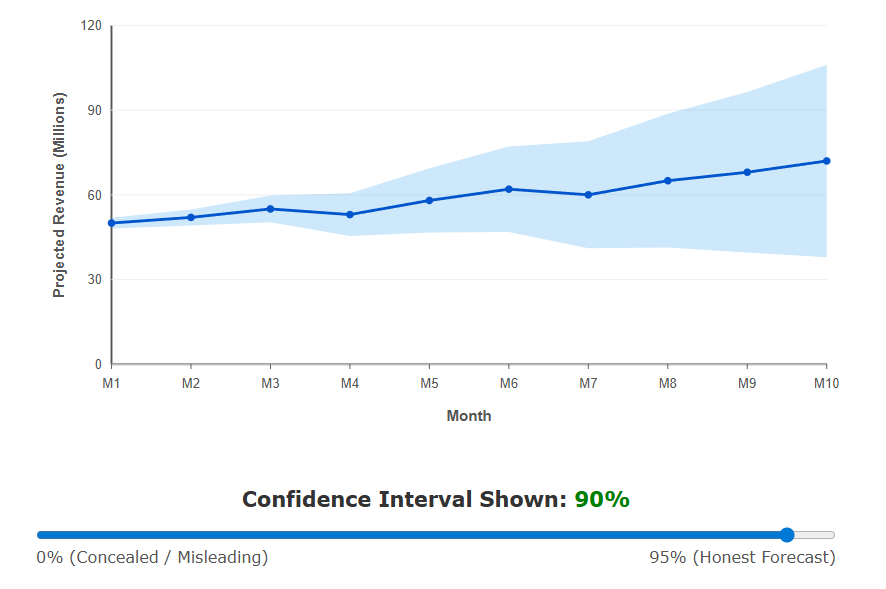
\includegraphics[width=0.8\textwidth]{images/Concealing_uncertainty_demo_example.png}
    \caption[Concealing Uncertainty Revenue Example.]{Screenshot created by authors from the interactive demo.}
    \label{fig:concealing_uncertainty}
\end{figure}

